\section{Results \& Discussion}\label{s:results}

\subsection{Variation In Indoor Air Contaminant Concentration Over Time}\label{s:results_variation_time}

High frequency measurement of indoor air contaminant concentrations, $c_\mathrm{in}$, such as those in Figure \ref{fig:indianapolis}, took place at both the ASU House and the Indianapolis House over significant periods (Indianapolis: ca 1.7 years, ASU house: ca 3.5 years)\cite{u.s._environmental_protection_agency_assessment_2015,holton_temporal_2013}.
Furthermore, at the Indianapolis site $c_\mathrm{in}$ for three different contaminants, chloroform, TCE, and tetrachloroethylene (PCE) were all collected, allowing examination of the variability of each VI contaminant.
The NAS North Island NAS dataset was obtained over a much shorter duration (9 days), and is therefore not examined in this portion of the analysis.
It should also be noted that the ASU house used 4-hour sorbent tubes, while Indianapolis took instantaneous "grab" samples.\par

Figure \ref{fig:indianapolis} showed a large degree of temporal variation in one of the components, and the data for the other components were quite similar.
What is apparent upon closer examination of such data is that the actual day-to-day variations are typically not nearly as large as those observed when tracking the data for a longer time.
To demonstrate this point, the quotient of the maximum and minimum $c_\mathrm{in}$ values (denoted as $c_\mathrm{max}/c_\mathrm{min}$) are shown as a function of time in Figure \ref{fig:resampling}.
The values shown in Figure \ref{fig:resampling} are the means of the quotients calculated for samples separated by the indicated times and the error bars indicate the 95th percentile of all the data points.
Hypothetical resampling periods of one, two, three days, and the same number of weeks, and months were chosen.\par

\begin{figure}[htb!]
 \centering
 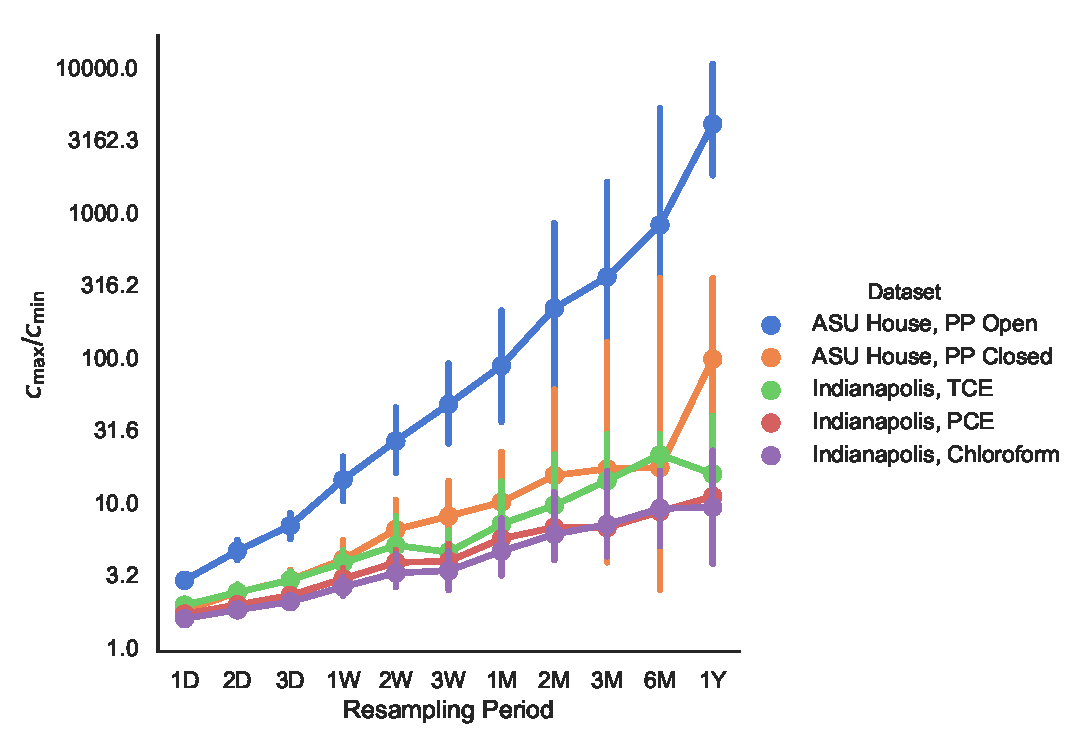
\includegraphics[width=\textwidth]{resampling.pdf}
 \caption{Mean values of the maximum change in indoor air contaminant concentration that may be expected over a given time period. (e.g., 1D is 1 day, 2W is 2 weeks, and 3M is 3 months). The error bars are the 95\% confidence intervals.}\label{fig:resampling}
\end{figure}

For example, if the data are examined in terms of the mean maximum variation observable over the course of 24 hours (one day) the variation is no greater than about a factor of two for any of the contaminants at the Indianapolis house or for TCE at the ASU house (when the preferential pathway was closed).
The mean variability at the latter was only a bit higher (about a factor of 3) when the preferential pathway was open.
In other words, a sampling protocol that involves sampling on two consecutive days would typically not uncover the large temporal variations that characterize the site over longer periods of time.
As Figure \ref{fig:indianapolis} shows, there are certainly isolated days in which a larger daily change was observed, but these were not typical, to the extent that they fall outside of the 95\% criteria used in defining the error bars.
So while such unusual jumps might be seen (for unknown reasons) in a very small percentage of cases, the expectation is much more represented by what is shown in Figure \ref{fig:resampling}.\par

Weeks of temporal separation in sampling events are required to observe the large variations of concern.
Orders of magnitude differences begin to manifest themselves over the course of months.
This is not surprising, since those who performed the measurements have already reported that there were seasonal aspects to the values obtained.
This would be consistent with requiring months to see the more significant variations.\par

This analysis also suggests that certain types of preferential pathways contribute to larger variations on shorter timescales (ASU House).
Even though there was a preferential pathway present at the Indianapolis House, the transients associated with its presence were of a slower nature and the behavior was not unlike what was observed at ASU House when the preferential pathway was closed.
This warns that the mere existence of a preferential pathway is not by itself sufficient to create a situation of large variations over short sampling times.\par

The longer the resampling period, the larger the maximum variability in observed indoor air contaminant concentrations.
In the case of the ASU House with the preferential pathway open, the variability went from less than a threefold difference on the timescale of a day, to two to three orders of magnitude over the course of weeks.
Thus there are different timescales that characterize different extents of variation, again pointing to the existence of more than a single factor that determines variability.\par

Multiple samples taken over a short time period, e.g. a few days, are unlikely to uncover significant variation in indoor air contaminant concentration; the larger transient variations typically manifest after longer time periods. \par

\subsection{Statistical Analysis of Field Data}\label{s:results_pressure_concentration}

The data in Figure \ref{fig:indianapolis} and Figure \ref{fig:resampling} raise the question of what then actually determines the large degree of temporal variation sometimes reported.
The rate of advective entry of soil gas into a structure is frequently cited as playing an important role in determining entry rate of contaminant.
This advective entry rate is closely linked to the indoor-outdoor pressure difference, as can be caused by the “stack effect”, for example.
Thus we first consider how much variability there might be in the pressure driving force for advection, and if this can explain the observed variability in observed indoor air contaminant concentrations.\par

The pressure difference between the indoor and outdoor/ambient ($p_\mathrm{in/out}$) leads to advection, by which contaminants are drawn into (or prevented from) entering a structure. 
Changes in $p_\mathrm{in/out}$ can take place quickly, leaving open the possibility of their impacting VI far more rapidly than can fluctuations in say groundwater depth or contaminant concentration (these latter processes take weeks or even months to impact the overlying structure).\par

We examine the relationship between $p_\mathrm{in/out}$ and $c_\mathrm{in}$ by constructing the two-dimensional kernel density estimation (KDE) plots seen in Figure \ref{fig:kde}.
The KDE plots allow us to view the measured distributions of $p_\mathrm{in/out}$ and $c_\mathrm{in}$, and develop a visual impression of how well these distributions correlate with one another.
For this analysis we considered two VI sites, NAS North Island and the ASU House.
The ASU House dataset was divided into two periods, one before and the other after the land drain (called the preferential pathway (PP) from  here on) had been closed.
By comparing these two periods on a single plot, the impact of the preferential pathway becomes clearer.\par

\begin{figure}[htb!]
 \centering
 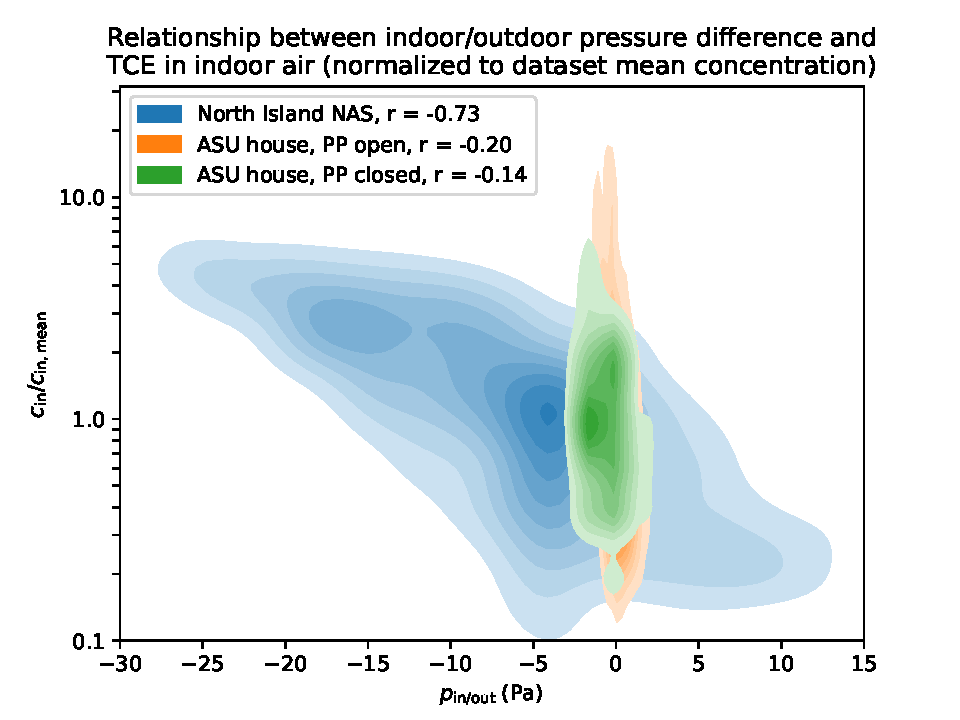
\includegraphics[width=\textwidth]{nas_asu_pp.pdf}
 \caption{2D-KDE plot showing the distributions of indoor air contaminant concentration, the indoor/outdoor pressure difference, and how they correlate to each other.}\label{fig:kde}
\end{figure}

\begin{table}[htb!]
  \newcommand{\NameEntry}[1]{
    \multicolumn{2}{c}{
      \multirow{2}{*}{
        \begin{minipage}{0.2\textwidth}
          \centering
          \textbf{#1}
        \end{minipage}
      }
    }
  }
  \centering
  \begin{tabular}{c c c c c c c}
    \toprule
    \multirow{2}{*}{ } & \NameEntry{North Island NAS} & \NameEntry{ASU House PP Open} & \NameEntry{ASU House PP Closed} \\ \\
    \midrule
    Percentile & 5th & 95th & 5th & 95th & 5th  & 95th \\
    $p_\mathrm{in/out}$ (Pa) & -19.9 & 7.4 & -1.4 & 2.1  & -2.1 & 2.27 \\
    $c_\mathrm{in}/c_\mathrm{in,mean}$ & 4.1 & 0.2 & 13.5 & 0.2  & 3.3  & 0.4  \\
    \bottomrule
  \end{tabular}
 \caption{5th and 95th percentile values of $p_\mathrm{in/out}$ and $c_\mathrm{in}/c_\mathrm{in,mean}$ in Figure \ref{fig:kde}.}\label{tbl:percentiles}
\end{table}

In Figure \ref{fig:kde}, the indoor air contaminant concentration $c_\mathrm{in}$ is normalized to the mean $c_\mathrm{in,mean}$ of each dataset, allowing comparison of the impact $p_\mathrm{in/out}$ on $c_\mathrm{in}$ independently from the large differences in absolute values of indoor air concentrations at the different sites.
A value of 10 on the y-axis indicates that the corresponding plotted value of $c_\mathrm{in}$ is 10 times greater than the mean for the dataset, and 0.1 indicate that it is one tenth of the mean.\par

Inspection of the range of normalized $c_\mathrm{in}$ values in Figure \ref{fig:kde} again shows the two order of magnitude spread in observed values, implying a sampling at one particular time might give a value that is two orders of magnitude different than a result from a different time.
Such issues have of course already been pointed out by the investigators who obtained the data.\par

The power of this KDE representation is that it permits evaluation of the relationship of two independently measured data - the indoor air contaminant concentration and the indoor-outdoor pressure difference.
Examining the data in this manner immediately points to an important difference between the data from the ASU House and those from NAS North Island.
At NAS North Island site $p_\mathrm{in/out}$ varies significantly; the 5th and 95th percentile of $p_\mathrm{in/out}$ are -19.9 and 7.4 Pa respectively.
This may be contrasted with 5th and 95th percentile $p_\mathrm{in/out}$ at the ASU house: -1.4 and 2.1 Pa (with the PP open), and -2.1 and 2.27 Pa (PP closed).\par

The much larger under- and overpressurization of the NAS North Island site compared to the ASU House makes the pressure dependence of indoor air concentration much more visible at the former site.
The Pearson’s r-value for the correlation between $p_\mathrm{in/out}$ and $c_\mathrm{in}$ for each dataset is shown in the legend, and confirms what is apparent to the eye; the pressure driving force is a determining factor for observed contamination at NAS North Island.
But the broadness of the band of the NAS North Island concentration data set suggests that there is still a source of variability in $c_\mathrm{in}$ that has not been fully captured - this will be addressed below.\par

The ASU house datasets offer a different picture.
The variability of $c_\mathrm{in}$ is just as large, or even larger than at NAS North Island, yet the $p_\mathrm{in/out}$ varied far less.
The weaker dependence of $c_\mathrm{in}$ on the pressure difference is confirmed by the much lower r-values for the correlations between the variables.
In other words, there is not nearly as strong a correlation between variation in indoor air contaminant concentration and pressure difference for the ASU House as there was for NAS North Island.
These results strongly suggest that there are other factors besides indoor pressure determining indoor air contaminant concentrations, and their variations, that may not be accounted for in applying this method.\par

The data for the ASU House also offer an insight into the role of the preferential pathway.
At first glance it may seem like the $c_\mathrm{in}$ values for the periods when the PP is open and closed are relatively comparable.
However, the 5th and 95th percentiles values of $c_\mathrm{in}$/$c_\mathrm{in,mean}$ differ significantly as may be seen in Table \ref{tbl:percentiles}.
It is clear that existence of the preferential pathway dramatically increases the variability in indoor air contaminant concentration.
This again is entirely consistent with what the investigators of that site have already reported\cite{guo_identification_2015}.
The correlation with indoor-outdoor pressure difference is weak in the ASU house cases, so there are clearly factors other than pressure difference that determine the variability in each.
These will be explored with the help of a modeling analysis presented below.\par

\subsection{Variability Of Attenuation to Subslab Concentrations}\label{s:results_attenuation}

Observed temporal variations in indoor air contaminant concentrations might be explained by temporal variations in subslab contaminant concentrations.
To examine how variability in subslab contaminant concentration might contribute to variability in indoor air contaminant concentration, data on the attenuation from subslab ($\alpha_\mathrm{subslab} = c_\mathrm{in}/c_\mathrm{subslab}$) were examined.
The dataset utilized for this was that from the ASU House.
The $c_\mathrm{subslab}$ values were taken from a soil gas probe labeled as "6" at the ASU house.
This probe was located closest to both the exit of the preferential pathway pipe, and to a reported breach in the foundation that served as a key entry pathway for contaminant getting into the house\cite{guo_identification_2015}.
The results are shown in Figure \ref{fig:attenuation_subslab}, which shows the full distributions for both the case in which the preferential pathway was "open" and when it "closed".\par

\begin{figure}[htb!]
  \centering
 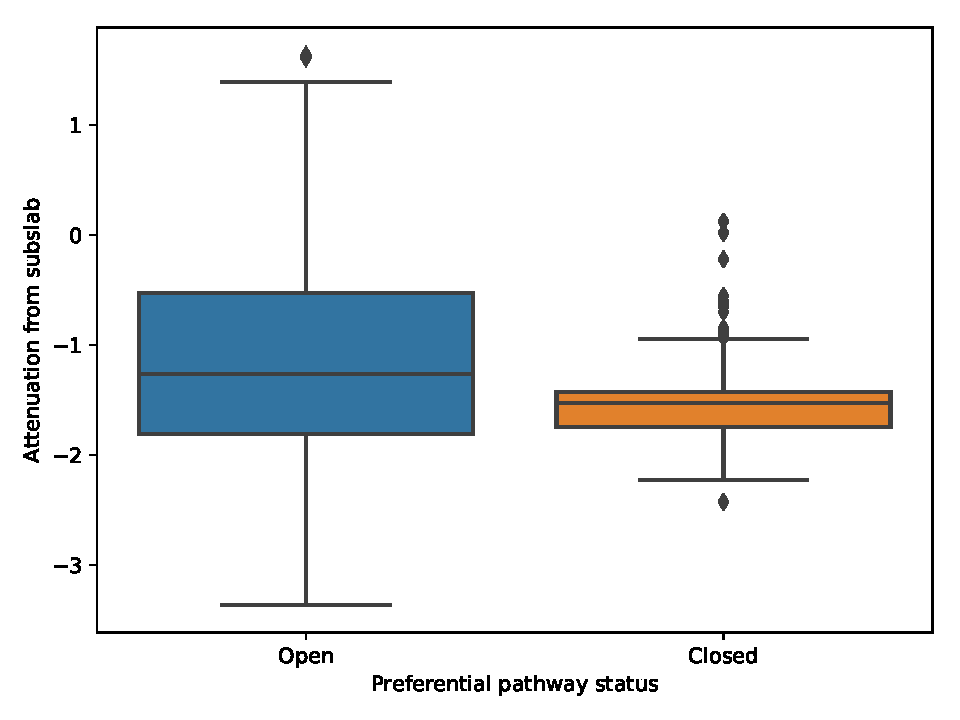
\includegraphics[width=0.7\textwidth]{asu_attenuation_subslab.pdf}
 \caption{Boxplot of $\log_{10}$ (subslab to indoor air contaminant attenuation) at the ASU house site. The box shows the quartiles of the distribution, the whiskers the extent of the distribution.}\label{fig:attenuation_subslab}
\end{figure}

It is apparent that during the period when the preferential pathway was closed, $\alpha_\mathrm{subslab}$ did not vary significantly, and was quite close to the EPA recommended $\alpha_\mathrm{subslab}$ value of 0.03\cite{u.s._environmental_protection_agency_oswer_2015}.
Thus during the period when the preferential pathway was closed, large temporal variations in subslab concentrations could not have been driving the variations in indoor air contaminant concentrations.\par

When the PP was open, there was considerably more variability in the subslab concentration values, and the mean value was higher than in the case where the preferential pathway was closed.
It was also not uncommon for the observed $\alpha_\mathrm{subslab}$ to exceed unity.
While large $\alpha_\mathrm{subslab}$ values may sometimes indicate indoor sources at a site, there were none at the ASU house.
A more likely explanation is that even though probe "6" was located in close proximity to the exit of the preferential pathway, there might have still existed significant spatial variability in $c_\mathrm{subslab}$ that could not be captured with a single measurement.
This suggests caution is needed in profiling subslab contaminant concentrations in the presence of preferential pathways - significant variations are possible.\par

What the results of Figure \ref{fig:attenuation_subslab} do clearly show is that the existence of a preferential pathway of the kind at ASU House (and idealized in Figure \ref{fig:indianapolis}) can influence the temporal variation of subslab concentrations in a much less predictable way than those observed in "normal" VI scenarios.\par

\subsection{Modeling Results}\label{s:results_model}

\subsubsection{Pressure Effects}\label{s:results_model_pressure}

Having established the potential impacts of certain inputs on determining variability in indoor air contaminant concentrations, the mathematical model of VI can help further elucidate other key aspects.
The results of calculations on a scenario corresponding to Figure \ref{fig:model} are presented in Figure \ref{fig:land_drain_scenarios}.
This scenario is not intended to exactly represent the situation at ASU House, but it is similar in the key aspect of having a preferential pathway delivering contaminant to a gravel sub-base.
The full, complex geometry of the ASU House has not been represented, but the modeled structure is of comparable size, and will be subject to operational parameters based upon what were measured at that site.
The general modeling conditions are those shown in Table \ref{fig:indianapolis}.\par

\begin{figure}[htb!]
 \centering
 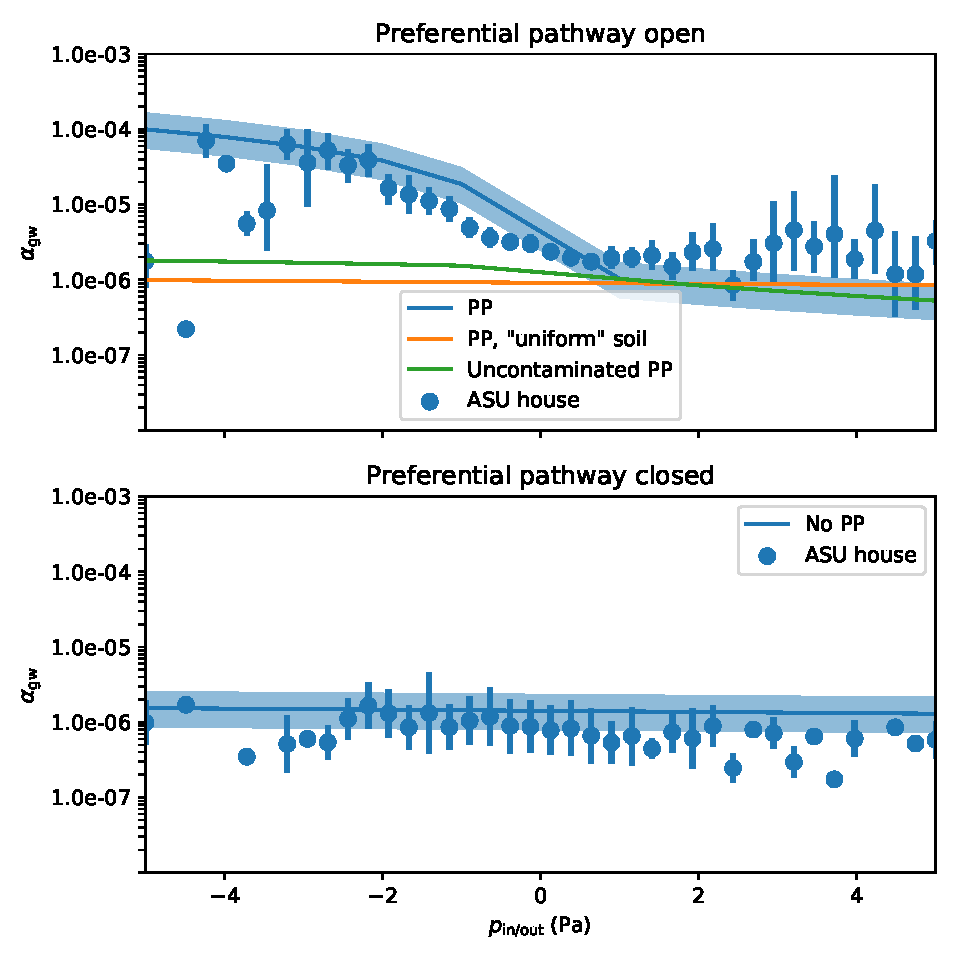
\includegraphics[width=\textwidth]{land_drain_scenarios_combo.pdf}
 \caption{Simulated preferential pathway scenarios compared to actual ASU house field data. Field data are binned in 40 evenly spaced pressure bins, with the dot representing the mean and errors bars the 95\% confidence interval of data at a particular pressure range. Shaded blue represent the range of model predictions for the indicated pressure difference, due to air exchange rate variability (using 5th and 95th percentile values of measured exchange rates). Top panel is for various cases representing an "open" preferential pathway, the lower panel with the pathway "closed".}\label{fig:land_drain_scenarios}
\end{figure}

In the calculation results shown in the top panel of Figure \ref{fig:land_drain_scenarios}, a preferential pathway is assumed to provide air containing contaminant vapor at a concentration equivalent to the vapor in equilibrium with the underlying groundwater source.
Here, the indoor air exchange rate $A_e$ was assumed to be a constant 0.5 per hour, and $p_\mathrm{in/out}$ was varied from -5 to 5 Pa.
Values of predicted indoor air contaminant concentrations, $c_\mathrm{in}$ were obtained from steady state calculations.
The predicted $c_\mathrm{in}$ values were then normalized by the assumed vapor concentration in equilibrium with groundwater $c_\mathrm{gw}$, giving the attenuation from groundwater $\alpha_\mathrm{gw}$.
The predicted values of $\alpha_\mathrm{gw}$ as a function of $p_\mathrm{in/out}$ are given by the central blue line in the upper panel of Figure \ref{fig:land_drain_scenarios}.
These predicted values are compared to actual measured $\alpha_\mathrm{gw}$ values from the ASU House for the period during which the preferential pathway was open (blue points).\par

The model successfully predicts the observed trends in $\alpha_\mathrm{gw}$ as $p_\mathrm{in/out}$ decreases (increased depressurization) but somewhat underpredicts $\alpha_\mathrm{gw}$ as the house is overpressurized.
Most significantly, the model captures that even for a small increase in depressurization (0 to -5 Pa) a very large increase in $\alpha_\mathrm{gw}$ (two order of magnitude) can occur.\par

The asymmetry relative to the predictions for depressurization and overpressurization is due to two factors.
First, the preferential pathway acts not only as a source of contaminant vapor, but also  as a source of air to the subslab.
Because of the large resistance to soil gas flow in the surrounding soil, having a local source of air to support the increase of advective flow into the structure from the subslab region makes a large difference.\par

The above was proven by a second simulation, where the model was rerun with the preferential pathway present, but with the permeable (gravel) layer in the subslab removed and replaced by the surrounding soil (sandy loam).
This gave a ”uniform soil” scenario the results of which are shown as an orange line in the top panel of Figure \ref{fig:land_drain_scenarios}.
This simulation demonstrates that without a permeable subslab to effectively allow the ”advective potential” to be realized, existence of preferential pathway will actually not impact a VI site very much.
In order for a preferential pathway to significantly contribute to VI, this requires a scenario involving good advective communication between it the indoor environment.
These requirements were met at the ASU House.\par

A perhaps obvious second requirement is that the preferential pathway must deliver contaminant vapors to be impactful.
In another simulation, the permeable (gravel) subslab region was included, but the preferential pathway merely delivered clean air to the subslab.
The result of this simulation is shown as the green line in the top panel of Figure \ref{fig:land_drain_scenarios}.
This shows that while there was a lightly larger $\alpha_\mathrm{gw}$ compared to the ”uniform soil” scenario, it is nowhere near as significant as when the preferential pathway delivers contaminant vapors.
The contaminated and uncontaminated preferential  pathway scenarios (blue and green lines respectively) thus bound the range of $\alpha_\mathrm{gw}$ that would be observed for a given $p_\mathrm{in/out}$ depending on the contaminant vapor concentration in the preferential pathway.\par

The model is also able to capture the weak trend in $\alpha_\mathrm{gw}$ with $p_\mathrm{in/out}$ when a preferential pathway is absent, but when there still exists a permeable subslab region.
These results are shown in the bottom panel of Figure \ref{fig:land_drain_scenarios}.  
These results are again in agreement with what was observed at the ASU House when the preferential pathway was closed, i.e. that there was a much more modest variation in indoor air concentration, irrespective of pressure, when the preferential pathway was cut off.\par

The above simulations capture the trend in $\alpha_\mathrm{gw}$ with $p_\mathrm{in/out}$ but do not yet capture the full variability of the concentration results over the "most probable" portion of observed pressure distributions shown in Figure \ref{fig:kde} (which tend to be from -2 to +2 Pa).
The results of Figure \ref{fig:land_drain_scenarios} show a spread of almost an order of magnitude over this pressure range for the case of the "open" preferential pathway, and almost no spread at all when the preferential pathway is "closed".
Hence the predicted variability is roughly an order of magnitude too low, when considering only the influence of pressure.
There is a factor that tends to increase the spread of the data one additional order of magnitude beyond what was predicted by the base calculations of Figure \ref{fig:land_drain_scenarios}.
We believe that it is variations in air exchange rate, operating in concert with the natural variations in pressure differential, that explain the remaining variability.\par

\subsubsection{Air Exchange Rate Effects}\label{s:results_model_air_exchange}

Table \ref{tbl:air_exchange_rate} shows the observed variations in air exchange rates for the ASU House and Indianapolis House, compared with EPA’s summary of the distribution of typical residential air exchange rates\cite{u.s._epa_exposure_2011,m._d._koontz_estimation_1995}.
Examination of these distributions point in a clear direction for modifying the above model.
Instead of using a constant value of air exchange rate, as is customary, its values should be parameterized.
A higher air exchange would of course be associated with lower $c_\mathrm{in}$ and vice versa.
Moreover, $A_e$ may sometimes be correlated with $p_\mathrm{in/out}$.
Determining any general relationship between $A_e$ and $p_\mathrm{in/out}$ is difficult: the structure itself and weather phenomena have a significant effect on air exchange.
As the data in Figure \ref{fig:air_exchange_rate} show, there is no easily discernable correlation between these variables at the ASU site, though there is a hint of slight seasonal dependence.
Note: a relationship between $A_e$ and $p_\mathrm{in/out}$ may be established for larger $p_\mathrm{in/out}$ via the building leakage curves, which are widely used for heating, ventilation and air conditioning systems in construction.\par

\begin{figure}[htb!]
  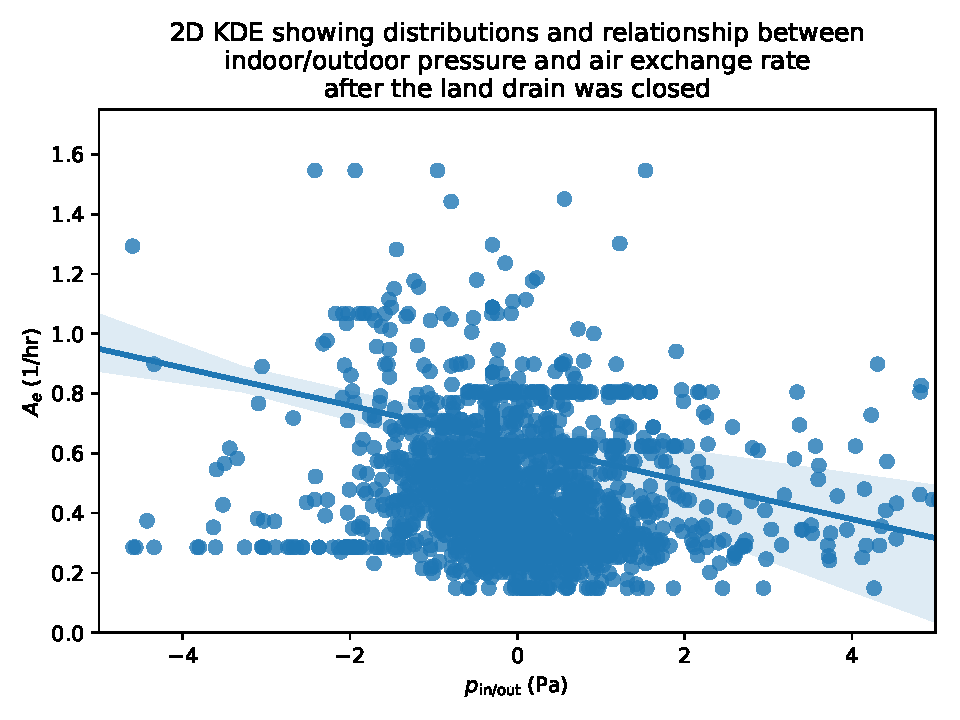
\includegraphics[width=\textwidth]{pressure_air_exchange_rate.pdf}
  \caption{2D KDE figure showing distributions and relationship between indoor/outdoor pressure difference and air exchange rate. The seasonal median $p_\mathrm{in/out}$ and $A_e$ are indicated by the location of the respective arrow tips. Only non-CPM period considered.}\label{fig:air_exchange_rate}
\end{figure}

\begin{table}[htb!]
  \centering
  \begin{tabular}{l c c c}
    \toprule
    \textbf{Percentile}                                                     & \textbf{10th} & \textbf{50th} & \textbf{90th} \\
    EPA\cite{u.s._epa_exposure_2011,m._d._koontz_estimation_1995}           & 0.16-0.2      & 0.35-0.49     & 1.21-1.49     \\
    ASU house\cite{holton_temporal_2013,guo_identification_2015}            & 0.21          & 0.43          & 0.78          \\
    Indianapolis\cite{u.s._environmental_protection_agency_assessment_2015} & 0.34          & 0.74          & 1.27          \\
    \bottomrule
  \end{tabular}
  \caption{Air exchange rate values (1/hr)}\label{tbl:air_exchange_rate}
\end{table}

To show the influence of possible statistical fluctuations of air exchange rate on the predictions of $\alpha_\mathrm{gw}$ values, the scenarios of Figure \ref{fig:land_drain_scenarios} were rerun calculated using the 5th and 95th percentile measured $A_e$ values, 0.17 and 0.90 respectively (based upon the actual distributions in Figure S1), providing predicted upper and lower bounds for $\alpha_\mathrm{gw}$.
These bounds are indicated by the shaded blue regions around the center line calculated for an assumed constant $A_e$ of 0.5 per hour.\par

It is apparent that assuming variability in air exchange rate allows capturing most of the observed variability in $\alpha_\mathrm{gw}$.
We believe that this explains the portion of the variation in indoor air contaminant concentration data that cannot be explained by either existence of preferential pathways or by the range in indoor depressurization.
Thus, we believe that it is the interplay of preferential pathway conditions, with indoor pressure variations and normal air exchange rates that help to explain the observations of significant variations in reported indoor air contaminant concentrations.\par

\subsubsection{Results of Transient Simulations}\label{s:results_modeling_transient}

The above analyses have been conducted under simulated steady state conditions.
The conclusions regarding the importance of the different parameters are now examined in actual transient simulations.
The model configuration of Figure \ref{fig:model} is run in 24-hour transient simulations to examine how $c_\mathrm{in}$ fluctuates over the course  of a "typical" day.
The simulations vary $p_\mathrm{in/out}$ as one model input, and then assume either a constant or time-varying air exchange rate, $A_e$.
The ASU House dataset was again the source of the "typical" $p_\mathrm{in/out}$ temporal variation, obtained by examining the median, hourly, diurnal $p_\mathrm{in/out}$ during the non-CPM periods.
The statistically "typical" $p_\mathrm{in/out}$ cycle may be seen in the upper left panel of Figure \ref{fig:diurnal} (note that values between the hourly median values are interpolated using cubic splines).
The "typical" air exchange rate is calculated in exactly the same way and is shown by the blue line in the upper right panel of Figure \ref{fig:diurnal}.
The orange line is the air exchange rate value assumed for the calculations at constant air exchange rate.\par

\begin{figure}
  \centering
 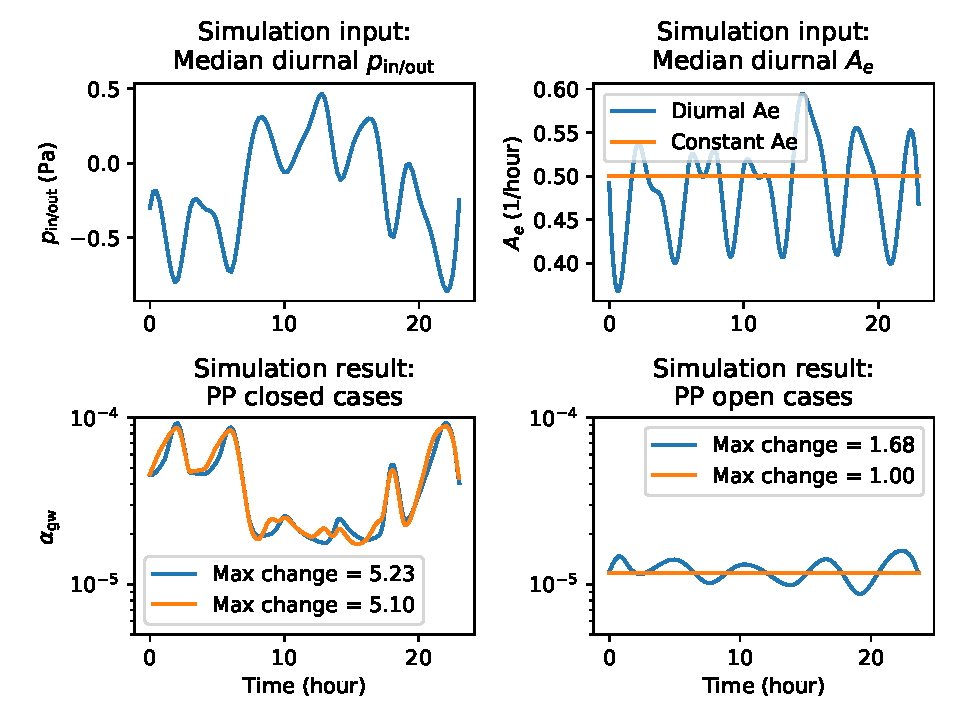
\includegraphics[width=\textwidth]{diurnal.pdf}
 \caption{Transient simulation of a "typical" VI day, using diurnal indoor/outdoor pressure difference and air exchange rate as inputs. Effect of preferential pathway considered.}\label{fig:diurnal}
\end{figure}

The result of these simulations are shown in the bottom two panels of Figure \ref{fig:diurnal}, where the left and right panels show the results of open and closed preferential pathways, respectively.
The "max change" value in the legends is the quotient of the lowest and highest predicted concentrations, i.e. a value of two indicate that the maximum daily concentration is twice as high as the lowest.
This quantity may be compared with the value that is plotted for "one day" in Figure \ref{fig:resampling}.
When the preferential pathway is open, there is a maximum daily variation of roughly a factor of 5, irrespective of whether $A_e$ fluctuates or not, which is somewhat more than the maximum daily variation shown in Figure \ref{fig:resampling}.
The relatively small difference between the variable and constant $A_e$ cases indicates that most of the variability during a "typical" day is here attributable to fluctuations in $p_\mathrm{in/out}$, i.e. the contaminant transport into the modeled structure is advection dominated.
Even for the small fluctuations in $p_\mathrm{in/out}$ the contaminant entry rate fluctuation drives the observed indoor concentration.
When the preferential pathway is closed the story is quite different.
When air exchange rate is held constant, there is essentially no variation in $c_\mathrm{in}$.
This is again not surprising, as Figure \ref{fig:land_drain_scenarios} demonstrated that when the preferential pathway is closed, the influence of $p_\mathrm{in/out}$ on contaminant entry rate (and subsequently $c_\mathrm{in}$) is small.
Combined with the small $p_\mathrm{in/out}$ this indicates that the contaminant transport into the modeled structure in this scenario is dominated by diffusion.
When the air exchange rate is allowed to fluctuate, the maximum daily variation in $c_\mathrm{in}$ is 1.68, which is in line with what is shown in Figure \ref{fig:resampling}.
This shows that for a "typical" day, when the preferential pathway is closed off, much of the daily variation in $c_\mathrm{in}$ is due to daily fluctuations in air exchange rate.\par

These results demonstrate the complicated nature of temporal variability in $c_\mathrm{in}$.
It is important to recall that only the effects of indoor/outdoor pressure difference and air exchange rate have been considered here, but slower processes, e.g. changes in groundwater contaminant concentration or various seasonal effects can also have a significant impact on VI over time.
For the shorter time periods of concern in recent studies of temporal variability in indoor contaminant concentrations we believe that these are dominated by combinations of indoor/outdoor pressure differentials and air exchange rate.
For a site where advective communication between the subsurface and the indoor is good, $p_\mathrm{in/out}$ is likely a significant determinant of $c_\mathrm{in}$ and its temporal variability.
We have shown that that such a scenario may arise due to a preferential pathway entering a permeable sub-base, but may also exist even in the absence of a preferential pathway just as the results from NAS North Island demonstrate.
At sites where advective transport into the structure is limited, much of the temporal variability in $c_\mathrm{in}$ may be attributed to natural fluctuations in air exchange rate.\par
